\documentclass{article}\usepackage{graphicx, color}
%% maxwidth is the original width if it is less than linewidth
%% otherwise use linewidth (to make sure the graphics do not exceed the margin)
\makeatletter
\def\maxwidth{ %
  \ifdim\Gin@nat@width>\linewidth
    \linewidth
  \else
    \Gin@nat@width
  \fi
}
\makeatother

\definecolor{fgcolor}{rgb}{0.2, 0.2, 0.2}
\newcommand{\hlnumber}[1]{\textcolor[rgb]{0,0,0}{#1}}%
\newcommand{\hlfunctioncall}[1]{\textcolor[rgb]{0.501960784313725,0,0.329411764705882}{\textbf{#1}}}%
\newcommand{\hlstring}[1]{\textcolor[rgb]{0.6,0.6,1}{#1}}%
\newcommand{\hlkeyword}[1]{\textcolor[rgb]{0,0,0}{\textbf{#1}}}%
\newcommand{\hlargument}[1]{\textcolor[rgb]{0.690196078431373,0.250980392156863,0.0196078431372549}{#1}}%
\newcommand{\hlcomment}[1]{\textcolor[rgb]{0.180392156862745,0.6,0.341176470588235}{#1}}%
\newcommand{\hlroxygencomment}[1]{\textcolor[rgb]{0.43921568627451,0.47843137254902,0.701960784313725}{#1}}%
\newcommand{\hlformalargs}[1]{\textcolor[rgb]{0.690196078431373,0.250980392156863,0.0196078431372549}{#1}}%
\newcommand{\hleqformalargs}[1]{\textcolor[rgb]{0.690196078431373,0.250980392156863,0.0196078431372549}{#1}}%
\newcommand{\hlassignement}[1]{\textcolor[rgb]{0,0,0}{\textbf{#1}}}%
\newcommand{\hlpackage}[1]{\textcolor[rgb]{0.588235294117647,0.709803921568627,0.145098039215686}{#1}}%
\newcommand{\hlslot}[1]{\textit{#1}}%
\newcommand{\hlsymbol}[1]{\textcolor[rgb]{0,0,0}{#1}}%
\newcommand{\hlprompt}[1]{\textcolor[rgb]{0.2,0.2,0.2}{#1}}%

\usepackage{framed}
\makeatletter
\newenvironment{kframe}{%
 \def\at@end@of@kframe{}%
 \ifinner\ifhmode%
  \def\at@end@of@kframe{\end{minipage}}%
  \begin{minipage}{\columnwidth}%
 \fi\fi%
 \def\FrameCommand##1{\hskip\@totalleftmargin \hskip-\fboxsep
 \colorbox{shadecolor}{##1}\hskip-\fboxsep
     % There is no \\@totalrightmargin, so:
     \hskip-\linewidth \hskip-\@totalleftmargin \hskip\columnwidth}%
 \MakeFramed {\advance\hsize-\width
   \@totalleftmargin\z@ \linewidth\hsize
   \@setminipage}}%
 {\par\unskip\endMakeFramed%
 \at@end@of@kframe}
\makeatother

\definecolor{shadecolor}{rgb}{.97, .97, .97}
\definecolor{messagecolor}{rgb}{0, 0, 0}
\definecolor{warningcolor}{rgb}{1, 0, 1}
\definecolor{errorcolor}{rgb}{1, 0, 0}
\newenvironment{knitrout}{}{} % an empty environment to be redefined in TeX

\usepackage{alltt}
\IfFileExists{upquote.sty}{\usepackage{upquote}}{}



\begin{document}

\title{The Hit and Run Algorithm}
\author{Mike Flynn}
\maketitle
To sample from the hull of a convex polytope, a random-walk algorithm
is typically used. The ``hit-and-run'' type algorithm uses the
following steps:

\begin{enumerate}
  \item Start from an intial solution $x_0$
  \item Pick a random direction in the polytope, $u$
  \item Isolate the segment $s$ connecting $x_0$ to a wall of the polytope
    in that direction $u$
  \item Sample uniformly from the segment $s$

\end{enumerate}


\noindent In Detail:
\\ \\
\noindent The polytope is defined as the set: ${x| Ax = A x_0, x \gt 0}$
where $x$ is a vector of length $n$, A is a $m \time n$ matrix of
constraints and $x_0$ an original solution. This set is geometrically
an intersection of $m$ n-planes defined by the rows of $A$ and the
half spaces $x_i \gt 0$. An easy case to picture is the 1-row A:
$[1,1,1]$ with initial solution $(.3,.3,.4)$. This corresponds the the
plane $x + y + z = 1$. The intersection of this plane with $x>0$
leaves only the part in the first octant, a triangle.

Because we must at another solution to $Ax = Ax_0$ in the end, picking
a ``random'' direction will not be a random direction in the space of
$x$ but rather a random direction in the k-plane that is
$Ax=Ax_0$. This is done by finding an orthogonal basis of the null
space of $A$: $Z_1, Z_2,\dots,Z_k$, which will necessarily be
orthogonal vectors in the k-plane. These basis vectors are weighted
uniformly by sampling their weights from an exponential distribution
and dividing by their sum. Therefore: $$ u = \sum_{j=0}^kZ_jr_j$$
where $r_j$ is the normalized random weight.

We sample along the segment $s$ by saying that $x_{i+1} = x_i + t*u$
where $t$ is some scalar parameter, bounded by the limits of
$s$. To sample uniformly on $s$, we merely must sample uniformly on
$t$, bounded by the limits of $s$. To find the limits of $t$ we must
simply recognize that for each index $i$: $$ x_i + t*u_i \gt 0 $$, of
which there are only 2 important cases: when $u_i \gt 0$ and when $u_i
< 0$. This is because when we solve for the limits of $t$ we simply
divide by $u_i$ to get 2 equations:

$$ t_i \gt -\frac{x_i}{u_i} \text{ for } u_i > 0 $$
$$ \text{and}$$
$$ t_i \lt -\frac{x_i}{u_i} \text{ for } u_i < 0 $$

Therefore the largest $t$ can be is large enough so that it is still
less than the smallest such right hand side for the second equation,
set by $x_i$, and likewise, must be greater than the largest right
hand side for the first equation. Formally:

$$  t_{\text{max}} = \text{Min}(-\frac{x_i}{u_i}) \text{ for } u_i < 0 $$
$$ \text{and}$$
$$  t_{\text{min}} = \text{Max}(-\frac{x_i}{u_i}) \text{ for } u_i > 0 $$

After these are figured out, $t$ can be drawn from a uniform
distribution between $t_{\text{min}}$ and $t_{\text{max}}$ to walk
randomly on the simplex.
\\ \\

\noindent A demonstration:

\begin{knitrout}
\definecolor{shadecolor}{rgb}{0.969, 0.969, 0.969}\color{fgcolor}\begin{kframe}
\begin{alltt}
\hlfunctioncall{require}(MASS)
\hlfunctioncall{require}(scatterplot3d)
\hlcomment{#' Uniformly samples from \{A*x=A*x0\} U \{x>0\}}
getWeights.hnr <- \hlfunctioncall{function}(A, x0, n, discard) \{
    
    y = x0
\hlcomment{    ## resolve weird quirk in Null() function}
    \hlfunctioncall{if} (\hlfunctioncall{ncol}(A) == 1) \{
        Z = \hlfunctioncall{Null}(A)
    \} else \{
        Z = \hlfunctioncall{Null}(\hlfunctioncall{t}(A))
    \}
    X = \hlfunctioncall{matrix}(0, nrow = \hlfunctioncall{length}(x0), ncol = n + discard)
    \hlfunctioncall{for} (i in 1:(n + discard)) \{
\hlcomment{        ## u is a random unit vector}
        u = \hlfunctioncall{rexp}(\hlfunctioncall{ncol}(Z))
        u = u/\hlfunctioncall{sum}(u)
        
\hlcomment{        ## d is a unit vector in the appropriate k-plane pointing in a random}
\hlcomment{        ## direction}
        d = Z %*% u
        c = y/d
\hlcomment{        ## determine intersections of x + t*d with edges}
        tmin = \hlfunctioncall{max}(-c[d > 0])
        tmax = \hlfunctioncall{min}(-c[d < 0])
        
\hlcomment{        ## writeLines(paste('tmin: ', tmin, '\textbackslash{}ntmax: ', tmax, '\textbackslash{}n', sep = ''))}
\hlcomment{        ## chose a point on the line segment}
        y = y + (tmin + (tmax - tmin) * \hlfunctioncall{runif}(1)) * Z %*% u
        X[, i] = y
    \}
    \hlfunctioncall{return}(X[, (discard + 1):\hlfunctioncall{ncol}(X)])
\}


\hlcomment{## Sample from the triangle \{x+y+z =1\} U \{x>0\}}
Amat = \hlfunctioncall{matrix}(\hlfunctioncall{c}(1, 1, 1), ncol = 3, nrow = 1)
x0 = \hlfunctioncall{c}(0.3, 0.2, 0.5)
w = \hlfunctioncall{getWeights.hnr}(Amat, x0, 1000, 5)

\hlfunctioncall{scatterplot3d}(x = w[1, ], y = w[2, ], z = w[3, ], angle = 160)
\end{alltt}
\end{kframe}
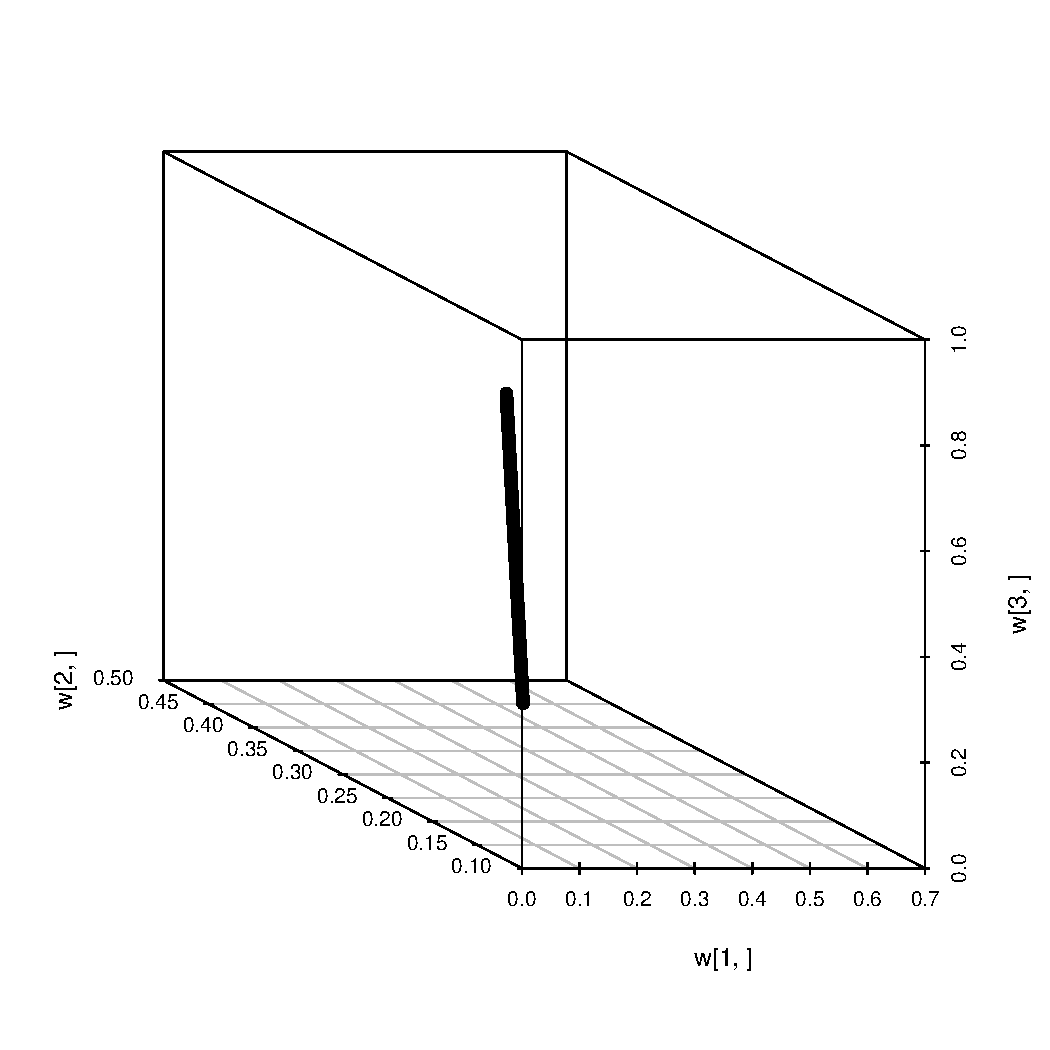
\includegraphics[width=\maxwidth]{figure/demo} 

\end{knitrout}


\end{document}
